\begin{name}
	{\tenchude}
	{\tendethi}
	{Sở Yên Bái}
	{\thoigian}
\end{name}
\Opensolutionfile{ans}[ans/2-TT-SoYenBai-L2-NH21-22]

%Câu 1-16: Vũ Ngọc Phát

%Câu 1
\begin{ex}%[Dự án 16 - TeamTeXHoa - TT SoYenBai - Vũ Ngọc Phát]%[2H2Y1-2]
Cho hình nón có bán kính đáy bằng $5$, độ dài đường sinh bằng $7$. Diện tích xung quanh của hình nón bằng
\choice
{$12\pi$}
{$175\pi$}
{$70\pi$}
{\True $35\pi$}
\loigiai{
$S_{\text{xq}}=\pi rl=\pi \cdot 5 \cdot 7 =35\pi$.
}
\end{ex}

%Câu 2
\begin{ex}%[Dự án 16 - TeamTeXHoa - TT SoYenBai - Vũ Ngọc Phát]%[1D3Y4-3]
Cho cấp số nhân $(u_n)$ có $u_1=-3$ và công bội $q=4$. Khi đó $u_2$ bằng
\choice
{\True $-12$}
{$\dfrac{4}{3}$}
{$12$}
{$-\dfrac{3}{4}$}
\loigiai{
Ta có $u_2=u_1 \cdot q=-3 \cdot 4=-12$.
}
\end{ex}



%Câu 3
\begin{ex}%[Dự án 16 - TeamTeXHoa - TT SoYenBai - Vũ Ngọc Phát]%[2D2Y5-1]
Nghiệm của phương trình $5^x=3$ là
\choice
{\True $x=\log_5 3$}
{$x=\log_3 5$}
{$x=\sqrt[3]{5}$}
{$x=\dfrac{3}{5}$}
\loigiai{
$5^x=3 \Leftrightarrow x=\log_5 3$.
}
\end{ex}



%Câu 4
\begin{ex}%[Dự án 16 - TeamTeXHoa - TT SoYenBai - Vũ Ngọc Phát]%[2H3Y3-1]
Trong KG $Oxyz$, véc-tơ nào dưới đây là một véc-tơ chỉ phương của đường thẳng đi qua gốc tọa độ $O$ và điểm $Q(4;-3;5)$?
\choice
{$\overrightarrow{u}=(4;3;5)$}
{\True $\overrightarrow{u}=(4;-3;5)$}
{$\overrightarrow{u}=(4;-3;-5)$}
{$\overrightarrow{u}=(-4;-3;5)$}
\loigiai{
Đường thẳng đi qua gốc tọa độ $O$ và điểm $Q(4;-3;5)$ có véc-tơ chỉ phương $\overrightarrow{u}=\overrightarrow{OQ}=(4;-3;5)$.
}
\end{ex}



%Câu 5
\begin{ex}%[Dự án 16 - TeamTeXHoa - TT SoYenBai - Vũ Ngọc Phát]%[2D1Y1-1]
Cho hàm số $y=x^3-3x^2$. Mệnh đề nào dưới đây đúng?
\choice
{Hàm số nghịch biến trên khoảng $(2;+\infty)$}
{Hàm số nghịch biến trên khoảng $(-\infty ;0)$}
{Hàm số đồng biến trên khoảng $(0;2)$}
{\True Hàm số nghịch biến trên khoảng $(0;2)$}
\loigiai{
$y=x^3-3x^2 \Rightarrow y'=3x^2-6x$.\\
$y'=0\Leftrightarrow \hoac{& x=0 \\& x=2}$.\\
Bảng biến thiên\\
\begin{center}

\begin{tikzpicture}[line join=round, line cap=round, >=stealth]
\tkzTabInit[nocadre=true,lgt=1.2,espcl=2,deltacl=0.6]
{$x$ /0.8, $f'(x)$ /0.8, $f(x)$ /2}
{$-\infty$,$0$,$2$,$+\infty$}
\tkzTabLine{ ,+,z,-,z,+, }
\tkzTabVar{-/ , +/ , -/ , +/ }
\end{tikzpicture}
\end{center}
Vậy hàm số $y=x^3-3x^2$ nghịch biến trên khoảng $(0;2)$.
}
\end{ex}



%Câu 6
\begin{ex}%[Dự án 16 - TeamTeXHoa - TT SoYenBai - Vũ Ngọc Phát]%[2H2Y1-1]
Cho khối trụ có chiều cao $h=5$ và bán kính đáy $r=3$. Thể tích của khối trụ đã cho bằng
\choice
{$30\pi $}
{\True $45\pi $}
{$15\pi $}
{$75\pi $}
\loigiai{
Ta có $V=\pi r^2 h=\pi \cdot 3^2 \cdot 5 = 45\pi$.
}
\end{ex}



%Câu 7
\begin{ex}%[Dự án 16 - TeamTeXHoa - TT SoYenBai - Vũ Ngọc Phát]%[2D2Y2-1]
Tập xác định $\mathscr{D}$ của hàm số $y=x^{\sqrt{3}}$ là
\choice
{$(-\infty ;0)$}
{$\mathbb{R}$}
{$\mathbb{R} \setminus \{0\}$}
{\True $\left(0;+\infty\right)$}
\loigiai{
Vì $\sqrt{3} \notin \mathbb{Z}$ nên điều kiện xác định của $y=x^{\sqrt{3}}$ là $x>0$.\\
Vậy tập xác định của hàm số $y=x^{\sqrt{3}}$ là $\mathscr{D}=(0;+\infty)$.
}
\end{ex}



%Câu 8
\begin{ex}%[Dự án 16 - TeamTeXHoa - TT SoYenBai - Vũ Ngọc Phát]%[2H1Y3-2]
Cho lăng trụ có diện tích đáy $3a^2$ và chiều cao bằng $4a$. Thể tích khối lăng trụ bằng
\choice
{$3a^3$}
{$a^3$}
{$4a^3$}
{\True $12a^3$}
\loigiai{
$V=B \cdot h=3a^2 \cdot 4a=12a^3$.
}
\end{ex}



%Câu 9
\begin{ex}%[Dự án 16 - TeamTeXHoa - TT SoYenBai - Vũ Ngọc Phát]%[2D1Y2-2]
Cho hàm số $f(x)$ liên tục trên $\mathbb{R}$ và có bảng xét dấu $f'(x)$ như sau
\begin{center}

\begin{tikzpicture}[line join=round, line cap=round]
\tkzTabInit[nocadre=true,lgt=1.2,espcl=2,deltacl=0.6]
{$x$ /0.8, $f'(x)$ /0.8}
{$-\infty$,$-1$,$0$,$1$,$3$,$+\infty$}
\tkzTabLine{ ,-,z,+,z,-,d,+,z,+, }
\end{tikzpicture}
\end{center}
Số điểm cực tiểu của hàm số là
\choice
{\True $2$}
{$3$}
{$4$}
{$1$}
\loigiai{
Vì đạo hàm của hàm số đổi dấu từ âm sang dương khi đi qua điểm cực tiểu nên dựa vào bảng xét dấu của $f'(x)$, hàm số $f(x)$ có $2$ điểm cực tiểu.
}
\end{ex}



%Câu 10
\begin{ex}%[Dự án 16 - TeamTeXHoa - TT SoYenBai - Vũ Ngọc Phát]%[2H3Y1-1]
Trong KG $Oxyz$, điểm nào sau đây nằm trên trục $Oz$?
\choice
{$B(0;2;0)$}
{\True $A(0;0;2)$}
{$D(1;2;3)$}
{$C(2;0;0)$}
\loigiai{
Ta có $A(0;0;2)$ nằm trên trục $Oz$.
}
\end{ex}



%Câu 11
\begin{ex}%[Dự án 16 - TeamTeXHoa - TT SoYenBai - Vũ Ngọc Phát]%[1D2Y2-1]
Cần chọn $2$ cái bút bi từ $15$ cái bút bi khác nhau. Khi đó số cách chọn là
\choice
{\True $\mathrm{C}_{15}^2$}
{$30$}
{$\mathrm{A}_{15}^2$}
{$2^{15}$}
\loigiai{
Có $\mathrm{C}_{15}^2$ cách chọn $2$ cái bút bi từ $15$ cái bút bi khác nhau.
}
\end{ex}



%Câu 12
\begin{ex}%[Dự án 16 - TeamTeXHoa - TT SoYenBai - Vũ Ngọc Phát]%[2D1Y3-1]
Giá trị nhỏ nhất của hàm số $f(x)=x^3-21x$ trên đoạn $[2;19]$ bằng
\choice
{$-34$}
{$14\sqrt{7}$}
{\True $-14\sqrt{7}$}
{$-36$}
\loigiai{
Ta có $f'(x)=3x^2-21$.\\
$f'(x)=0\Leftrightarrow \hoac{& x=\sqrt{7} \in (2;19) \\& x=-\sqrt{7} \notin (2;19)} $.\\
Có $f(2)=-34$, $f(\sqrt{7})=-14\sqrt{7}$, $f(19)=6460$.\\
Suy ra $ \min \limits_{[2;19]} f(x)=-14\sqrt{7}$.
}
\end{ex}



%Câu 13
\begin{ex}%[Dự án 16 - TeamTeXHoa - TT SoYenBai - Vũ Ngọc Phát]%[2D1Y1-2]
Cho hàm số $y=f(x)$ có bảng xét dấu đạo hàm như hình sau
\begin{center}

\begin{tikzpicture}[line join=round, line cap=round, >=stealth]
\tkzTabInit[nocadre=true,lgt=1,espcl=2,deltacl=0.6]
{$x$ /0.8, $y'$ /0.8}
{$-\infty$,$-1$,$1$,$+\infty$}
\tkzTabLine{ ,-,d,-,z,+, }
\end{tikzpicture}
\end{center}
Hàm số đã cho nghịch biến trên khoảng nào dưới đây?
\choice
{$(-\infty ;1)$}
{$(1;+\infty)$}
{$(-1;+\infty)$}
{\True $(-\infty ;-1)$}
\loigiai{
}
\end{ex}



%Câu 14
\begin{ex}%[Dự án 16 - TeamTeXHoa - TT SoYenBai - Vũ Ngọc Phát]%[2D3Y1-1]
Cho hàm số $f(x)=1-\cos x$. Khẳng định nào sau đây đúng?
\choice
{$\displaystyle\int f(x) \mathrm{\,d}x =x+\sin x+C$}
{\True $\displaystyle\int f(x) \mathrm{\,d}x =x-\sin x+C$}
{$\displaystyle\int f(x)\mathrm{\,d}x =\sin x+C$}
{$\displaystyle\int f(x)\mathrm{\,d}x =-\sin x+C$}
\loigiai{
Ta có $\displaystyle\int f(x)\mathrm{\,d}x =x-\sin x+C$.
}
\end{ex}



%Câu 15
\begin{ex}%[Dự án 16 - TeamTeXHoa - TT SoYenBai - Vũ Ngọc Phát]%[2D4Y1-1]
Số phức $z=3-4i$ có phần ảo là
\choice
{$-4i$}
{$4i$}
{$4$}
{\True $-4$}
\loigiai{
Số phức $z=3-4i$ có phần ảo là $-4$.
}
\end{ex}


%Câu 16
\begin{ex}%[Dự án 16 - TeamTeXHoa - TT SoYenBai - Vũ Ngọc Phát]%[2D4Y1-2]
Trên mặt phẳng tọa độ, điểm biểu diễn số phức $2+i$ có tọa độ là
\choice
{$(-2;1)$}
{\True $(2;1)$}
{$(1;2)$}
{$(2;-1)$}
\loigiai{
Trên mặt phẳng tọa độ, điểm biểu diễn số phức $2+i$ có tọa độ là $(2;1)$.
}
\end{ex}

%Câu 17
\begin{ex}%[Dự án giải đề Sở GD, Bùi Anh Tuấn]%[2H3Y1-3]
	Trong KG $Oxyz$, cho mặt cầu $(S)\colon x^2+y^2+z^2+4x-2y+8z+17=0$. Tọa độ tâm $I$ và bán kính $R$ của mặt cầu $(S)$ là
	\choice
	{$I(-2;1;-4), R=4$ }
	{\True $I(2;-1;4), R=2$}
	{$I(2;-1;4), R=4$}
	{\True$I(-2;1;-4), R=2$}
	\loigiai{
		Mặt cầu $(S)$ có tâm $I(-2;1;-4)$, bán kính $R=\sqrt{(-2)^{2}+1^{2}+(-4)^{2}-17}=2$.}
\end{ex}

\begin{ex}%[Dự án giải đề Sở GD, Bùi Anh Tuấn]%[2H2Y2-1]
	Cho mặt cầu có đường kính bằng $6$. Diện tích $S$ của mặt cầu đã cho bằng
	\choice
	{$72\pi $}
	{$18\pi $}
	{\True $36\pi $}
	{$144\pi $}
	\loigiai{
		Mặt cầu đã cho có bán kính bằng $3$.\\
		Diện tích $S$ của mặt cầu đã cho bằng 
		$S=4\pi\cdot R^2=4\pi\cdot 3^2=36\pi$.
	}	
\end{ex}

\begin{ex}%[Dự án giải đề Sở GD, Bùi Anh Tuấn]%[2D3Y2-1]
	Nếu $\displaystyle\int\limits_0^2 f(x)\mathrm{\,d}x=-4$ và $\displaystyle\int\limits_0^2 g(x)\mathrm{\,d}x=5$ thì $\displaystyle\int\limits_0^2 \left[f(x)+g(x)\right] \mathrm{\,d}x$ bằng
	\choice
	{$9$}
	{$-9$}
	{$-1$}
	{\True $1$}
	\loigiai{
		Ta có $$\displaystyle\int\limits_0^2 \left[f(x)+g(x)\right] \mathrm{\,d}x
		=\displaystyle\int\limits_0^2 f(x)\mathrm{\,d}x + \displaystyle\int\limits_0^2 g(x)\mathrm{\,d}x=-4+5=1.$$
	}
\end{ex}

\begin{ex}%[Dự án giải đề Sở GD, Bùi Anh Tuấn]% [2D1B5-3] 
	\immini{Cho hàm số bậc ba $y=f(x)$ có đồ thị là đường cong trong hình bên.  Số nghiệm thực của phương trình $4f(x)-3=0$
		\choice
		{\True $3$}
		{$2$}
		{$1$}
		{$0$}}{
		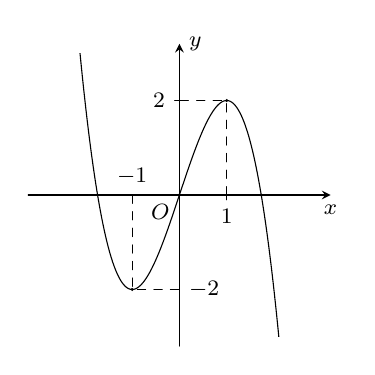
\begin{tikzpicture}[scale=.6, font=\footnotesize, line join=round, line cap=round, >=stealth]
			\def\xmin{-3}\def\xmax{3}\def\ymin{-3}\def\ymax{3}
			\draw[->] (\xmin-0.2,0)--(\xmax+0.2,0) node[below] {\footnotesize $x$};
			\draw[->] (0,\ymin-0.2)--(0,\ymax+0.2) node[right] {\footnotesize $y$};
			\draw (0,0) node [below left] {\footnotesize $O$};
			\draw (-1,0) node [above] {\footnotesize $-1$};
			\draw (0,-2) node [right] {\footnotesize $-2$};
			\foreach \x in {1}\draw (\x,0.1)--(\x,-0.1) node [below] {\footnotesize $\x$};
			\foreach \y in {2}\draw (0.1,\y)--(-0.1,\y) node [left] {\footnotesize $\y$};
			\clip (\xmin,\ymin) rectangle (\xmax,\ymax);
			\draw[smooth,samples=200,domain=\xmin:\xmax] plot (\x,{-1*((\x)^3)+0*((\x)^2)+3*(\x)+0});
			\draw[dashed] (0.0,0)--(0.0,0.0)--(0,0.0);\fill (0.0,0.0) circle (1pt);
			\draw[dashed] (-1.0,0)--(-1.0,-2.0)--(0,-2.0);\fill (-1.0,-2.0) circle (1pt);
			\draw[dashed] (1.0,0)--(1.0,2.0)--(0,2.0);\fill (1.0,2.0) circle (1pt);
		\end{tikzpicture}
	}
	\loigiai{
		\immini{Ta có $4f(x)-3=0\Leftrightarrow f(x)=\dfrac{3}{4}$.\\
			Dựa vào đồ thị hàm số ta thấy phương trình $4f(x)-3=0$ có $3$ nghiệm phân biệt.}{
			\begin{tikzpicture}[scale=.6, font=\footnotesize, line join=round, line cap=round, >=stealth]
				\def\xmin{-3.75}\def\xmax{3}\def\ymin{-3}\def\ymax{3}
				\draw[->] (\xmin-0.2,0)--(\xmax+0.2,0) node[below] {\footnotesize $x$};
				\draw[->] (0,\ymin-0.2)--(0,\ymax+0.2) node[right] {\footnotesize $y$};
				\draw (0,0) node [below left] {\footnotesize $O$};
				\draw (-1,0) node [above] {\footnotesize $-1$};
				\draw (0,-2) node [right] {\footnotesize $-2$};
				\foreach \x in {1}\draw (\x,0.1)--(\x,-0.1) node [below] {\footnotesize $\x$};
				\foreach \y in {2}\draw (0.1,\y)--(-0.1,\y) node [left] {\footnotesize $\y$};
				\clip (\xmin,\ymin) rectangle (\xmax,\ymax);
				\draw[smooth,samples=200,domain=\xmin:\xmax] plot (\x,{-1*((\x)^3)+0*((\x)^2)+3*(\x)+0});
				\draw[dashed] (0.0,0)--(0.0,0.0)--(0,0.0);\fill (0.0,0.0) circle (1pt);
				\draw[dashed] (-1.0,0)--(-1.0,-2.0)--(0,-2.0);\fill (-1.0,-2.0) circle (1pt);
				\draw[dashed] (1.0,0)--(1.0,2.0)--(0,2.0);\fill (1.0,2.0) circle (1pt);
				\draw[red] (-3.75,0.75)--(3,0.75);
				\draw (-2.85,0.7) node [above] {\footnotesize $y=\tfrac{3}{4}$};
				
			\end{tikzpicture}
		}
	}
\end{ex}

\begin{ex}%[Dự án giải đề Sở GD, Bùi Anh Tuấn]%[2D3B2-1]
	Nếu $\displaystyle\int\limits_{0}^{2} f(x)\mathrm{d}x=-3$ thì $\displaystyle\int\limits_{0}^{2} \left[3f(x)-2\right]\mathrm{d}x$ bằng
	\choice
	{$-7$}
	{$-11$}
	{\True $-13$}
	{$-9$}
	\loigiai{
		Ta có $\displaystyle\int\limits_{0}^{2} \left[3f(x)-2\right]\mathrm{d}x=3\displaystyle\int\limits_{0}^{2} f(x)\mathrm{d}x-2\displaystyle\int\limits_{0}^{2} \mathrm{d}x=-9-4=-13$.
	}
\end{ex}

\begin{ex}%[Dự án giải đề Sở GD, Bùi Anh Tuấn]%^[2D4B4-3] 
	Trong tập số phức, phương trình $z^4+3z^2-4=0$ có tập nghiệm là
	\choice
	{$\{1;\ 2i\}$}
	{$\{-1;\ 1\}$}
	{\True $\{-1;\ 1;\ 2i;\ -2i\}$}
	{$\{2;\ -2;\ i;\ -i \}$}
	\loigiai{
		Ta có $z^4+3z^2-4=0\Leftrightarrow \hoac{&z^2=1\\&z^2=-4}\Leftrightarrow \hoac{&z=\pm 1\\&z=\pm 2i.}$
	}
\end{ex}

\begin{ex}%[Dự án giải đề Sở GD, Bùi Anh Tuấn]%[2D4Y2-2]
	Cho hai số phức $z=-1-i$ và $w=4+2i$. Môđun của số phức $z\cdot\overline{w}$ bằng
	\choice
	{$2\sqrt{5}$}
	{$10\sqrt{2}$}
	{$\sqrt{10}$}
	{\True $2\sqrt{10}$}
	\loigiai{
		Ta có $z\cdot\overline{w}=(-1-i)(4-2i)=-6-2i\Rightarrow\left|z\cdot\overline{w}\right|=\sqrt{(-6)^2+(-2)^2}=2\sqrt{10}$.}
\end{ex}

\begin{ex}%[Dự án giải đề Sở GD, Bùi Anh Tuấn]%[2D1Y4-1]
	Tiệm cận ngang của đồ thị hàm số $y=\dfrac{2x+1}{x-1}$ là
	\choice
	{$y=-1$}
	{$y=1$}
	{$y=\dfrac{1}{2}$}
	{\True $y=2$}
	\loigiai{
		Ta có
		\begin{itemize}
			\item $\lim\limits_{x\to+\infty} y=\lim\limits_{x\to+\infty}\dfrac{2x+1}{x-1}=\lim\limits_{x\to+\infty}\dfrac{2+\dfrac{1}{x}}{1-\dfrac{1}{x}}=2$.
			\item $\lim\limits_{x\to-\infty} y=\lim\limits_{x\to-\infty}\dfrac{2x+1}{x-1}=\lim\limits_{x\to-\infty}\dfrac{2+\dfrac{1}{x}}{1-\dfrac{1}{x}}=2$.
		\end{itemize}
		Vậy đồ thị hàm số có tiệm cận ngang là đường thẳng $y=2$.}
\end{ex}

\begin{ex}%[Dự án giải đề Sở GD, Bùi Anh Tuấn]%[2D3B2-1]
	Tính $\displaystyle\int\limits_1^3\dfrac{\mathrm{\,d}x}{5x-4}=a\ln b$ với $a$ là số hữu tỷ và $b$ là số nguyên tố. Khi đó $a+b$ bằng
	\choice
	{$11$}
	{\True $\dfrac{56}{5}$}
	{$12$}
	{$\dfrac{54}{5}$}
	\loigiai{
		Ta có $\displaystyle\int\limits_1^3\dfrac{\mathrm{\,d}x}{5x-4}=\dfrac{1}{5}\ln |5x-4|\bigg|_1^3=\dfrac{1}{5}\left(\ln 11-\ln 1\right)=\dfrac{1}{5}\cdot\ln 11$.\\
		Suy ra $a=\dfrac{1}{5}$; $b=11\Leftrightarrow a+b=\dfrac{1}{5}+11=\dfrac{56}{5}$.}
\end{ex}

\begin{ex}%[Dự án giải đề Sở GD, Bùi Anh Tuấn]%[2D1B3-2]
	Gọi $m$ là giá trị nhỏ nhất của hàm số $y=x+\dfrac{4}{x}$ trên khoảng $(0;+\infty)$. Tìm $m$.
	\choice
	{\True $m=4$}
	{$m=1$}
	{$m=3$}
	{$m=2$}
	\loigiai{
		Ta có $y'=1-\dfrac{4}{x^2}$; $y'=0\Leftrightarrow 1-\dfrac{4}{x^2}=0\Leftrightarrow \left[\begin{array}{l}
			x=2 \in(0 ;+\infty) \\
			x=-2 \notin(0 ;+\infty).
		\end{array}\right.$\\
		Bảng biến thiên
		\begin{center}
			
\begin{tikzpicture}
				\tkzTab[nocadre=true,lgt=1.2,espcl=2.5,deltacl=0.6]
				{$x$/0.6, $y'$/0.6, $y$/2} 
				{$0$, $2$, $+\infty$} 
				{,-,0,+,} 
				{+/$+\infty$, -/ $4$, +/$+\infty$} 
			\end{tikzpicture}
		\end{center}
		Dựa vào bảng biến thiên ta thấy  $\min\limits_{x \in (0;+\infty)} f(x)=f(2)=4$.
	}
\end{ex}

\begin{ex}%[Dự án giải đề Sở GD, Bùi Anh Tuấn]%[2D2Y4-2]
	Đạo hàm của hàm số $y=\ln (7x-5)$ là
	\choice
	{$y'=\dfrac{1}{(7x-5)\ln 7}$}	
	{$y'=\dfrac{7}{(7x-5)\ln 7}$}
	{\True $y'=\dfrac{7}{7x-5}$}
	{$y'=\dfrac{1}{7x-5}$}
	\loigiai{
		Ta có $y'=\left[\ln (7x-5)\right]'=\dfrac{(7x-5)'}{7x-5}=\dfrac{7}{7x-5}$.
	}
\end{ex}

\begin{ex}%[Dự án giải đề Sở GD, Bùi Anh Tuấn]%[2H3B2-3]
	Trong KG $Oxyz$, cho điểm $N(1;-2;-3)$ và đường thẳng $(d)\colon \dfrac{x-4}{3}=\dfrac{y+1}{-2}=\dfrac{x-1}{4}$. Mặt phẳng đi qua $N$ và vuông góc với đường thẳng $(d)$ có phương trình là
	\choice
	{$3x-2y+4z-3=0$}
	{$3x-2y+4z+3=0$}	
	{\True $3x-2y+4z+5=0$}
	{$3x-2y+4z-5=0$}
	\loigiai{
		Do mặt phẳng vuông góc với đường thẳng $(d)$ ta chọn véc-tơ pháp tuyến của mặt phẳng cần tìm là $\overrightarrow{n}=\overrightarrow{u_d}=(3;-2;4)$ và đi qua $N(1;-2;-3)$ nên có phương trình $$3(x-1)-2(y+2)+4(z+3)=0\Leftrightarrow 3x-2y+4z+5=0.$$
	}
\end{ex}

\begin{ex}%[Dự án giải đề Sở GD, Bùi Anh Tuấn]%[2H1B3-2]
	Cho hình lăng trụ tam giác đều $ABC.A'B'C'$ có $AB=a\sqrt{6}$, góc giữa đường thẳng $A'C$ và mặt phẳng $\left(ABC\right)$ bằng $30^{\circ}$. Thể tích khối lăng trụ $ABC.A'B'C'$ bằng
	\choice
	{$\dfrac{9a^3\sqrt{3}}{4}$}
	{$\dfrac{a^3\sqrt{3}}{6}$}
	{\True $\dfrac{3a^3\sqrt{6}}{2}$}
	{$2a^3\sqrt{3}$}
	\loigiai{
		\immini{Ta có lăng trụ $ABC.A'{B}'{C}'$ đều nên $$ A{A}'\perp\left(ABC\right)\Rightarrow\left(A'C,\left(ABC\right)\right)=\widehat{A'CA}=30^\circ . $$
			Tam giác $A'AC$ vuông tại $A$ có $AA'=AC \cdot \tan{30^o}=a\sqrt{6} \cdot \dfrac{1}{\sqrt{3}}=a\sqrt{2}$ .\\
			Tam giác $ ABC$ đều cạnh $ a$ nên $S_{\Delta ABC}=\dfrac{\left(a\sqrt{6}\right)^2 \cdot \sqrt{3}}{4}=\dfrac{3a^2\sqrt{3}}{2}.$\\
			Vậy thể tích khối lăng trụ $ABC.A'B'C'$ là $$V_{ABC.A'{B}'{C}'}=AA' \cdot S_{\Delta ABC}=\dfrac{3a^3\sqrt{6}}{2}.$$}
		{\begin{tikzpicture}[font=\footnotesize, line join=round, line cap=round, >=stealth,scale=0.6]
				\def\x{1}
				\def\y{2}
				\path 
				(\x,\y) coordinate (A)
				(\x+6,\y) coordinate (C)	
				(\x+1.5,\y-2) coordinate (B)
				(\x,\y+6) coordinate (A')		
				($(B)+(A')-(A)  $) coordinate (B')		
				($ (C)+(A')-(A) $) coordinate (C')
				($ (B)!.5!(C) $) coordinate (H)
				
				;
				\draw (A)--(B)--(C) (A)--(A') (B)--(B') (C)--(C') (A')--(B')--(C')--(A') ;
				\draw[dashed] (A)--(C) (A')--(C) ;
				\foreach \x/\g in{A/180,B/-90,C/0,A'/-160,B'/-40,C'/0}
				\fill[black](\x) circle (1pt)
				($(\x)+(\g:5mm)$) node{\small $\x$};
				%\node at (1.5,1) {$a $};
				%\node at (5,2.3) {$ a $};
				%\node at (0.5,4) {$ \dfrac{3a}{2} $};
		\end{tikzpicture} }
	}
\end{ex}

\begin{ex}%[Dự án giải đề Sở GD, Bùi Anh Tuấn]%[2H3B1-3]
	Trong KG $Oxyz$, cho điểm $I\left(1;4;-3\right)$ và mặt phẳng $(P) \colon x+2y-2z+3=0$. Mặt cầu $(S)$ tâm $I$ và tiếp xúc với $(P)$ có phương trình là
	\choice
	{\True $\left(x-1\right)^2+\left(y-4\right)^2+\left(z+3\right)^2=36$}
	{$\left(x-1\right)^2+\left(y-4\right)^2+\left(z+3\right)^2=16$}
	{$\left(x-1\right)^2+\left(y-4\right)^2+\left(z+3\right)^2=25$}
	{$\left(x+1\right)^2+\left(y+4\right)^2+\left(z-3\right)^2=36$}
	\loigiai{
		Bán kính mặt cầu là
		$R=\mathrm{d}\left( I;(P)\right) =\dfrac{\left|\,1+2\cdot4-2\cdot\left(-3\right)+3\right|}{\sqrt{1^2+2^2+(-2)^2}}=6$.\\
		Phương trình mặt cầu là $\left(x-1\right)^2+\left(y-4\right)^2+\left(z+3\right)^2=36.$
	}
\end{ex}

% Câu 31 - 42: Dũng Lê

\begin{ex}%[Dự án 16 - TeamTeXHoa - Sở Yên Bái - Dũng Lê]%[2D2B3-2]
	Với mọi số $a$, $b$ dương thoả mãn $\log_2a^2-\log_2b=2$, khẳng định nào dưới đây đúng?
	\choice
	{$a=2b^2$}
	{$a=4b^2$}
	{$a^2=2b$}
	{\True $a^2=4b$}
	\loigiai{
		Ta có $\log_2a^2-\log_2b=2\Leftrightarrow\log_2\dfrac{a^2}{b}=2\Leftrightarrow\dfrac{a^2}{b}=4\Leftrightarrow a^2=4b$.
	}
\end{ex}

\begin{ex}%[Dự án 16 - TeamTeXHoa - Sở Yên Bái - Dũng Lê]%[2D2B3-2]
	Cho $a>0$ và $a\neq 1$, khi đó $\log_a\sqrt{a\sqrt[3]{a}}$ bằng
	\choice
	{$\dfrac{4}{3}$}
	{$\dfrac{5}{6}$}
	{$\dfrac{5}{3}$}
	{\True $\dfrac{2}{3}$}
	\loigiai{
		Ta có $\log_a\sqrt{a\sqrt[3]{a}}=\log_a\left(a\cdot a^{\frac{1}{3}}\right)^{\frac{1}{2}}=\log_a a^{\frac{2}{3}}=\dfrac{2}{3}$.
	}
\end{ex}

\begin{ex}%[Dự án 16 - TeamTeXHoa - Sở Yên Bái - Dũng Lê]%[2D2B6-1]
	Tập nghiệm của bất phương trình $\log_3(x+2)>2$ là
	\choice
	{$(-2;7)$}
	{\True $(7;+\infty)$}
	{$(-2;+\infty)$}
	{$(-\infty;7)$}
	\loigiai{
		Ta có $\log_3(x+2)>2\Leftrightarrow x+2>9\Leftrightarrow x>7$.
	}
\end{ex}

\begin{ex}%[Dự án 16 - TeamTeXHoa - Sở Yên Bái - Dũng Lê]%[1H3K3-3]
	Cho hình chóp $S.ABCD$ có đáy $ABCD$ là hình vuông cạnh bằng $1$, $SA\perp (ABCD)$ và $SA=\sqrt{6}$. Góc giữa $SC$ và mặt phẳng $(ABCD)$ bằng
	\choice
	{$90^\circ$}
	{$30^\circ$}
	{\True $60^\circ$}
	{$45^\circ$}
	\loigiai{
		\immini{
			Vì $SA\perp(ABCD)$, nên $(SA,(ABCD))=\widehat{SAC}$.\\
			Ta có $AC=\sqrt{AD^2+CD^2}=\sqrt{2}$.\\
			Trong tam giác $SAC$ vuông tại $A$ có $\tan\widehat{SCA}=\dfrac{SA}{AC}=\sqrt{3}$.\\
			Suy ra $\widehat{SCA}=60^\circ$.\\
			Vậy góc giữa $SC$ và mặt phẳng $(ABCD)$ bằng $60^\circ$.
		}{
			\begin{tikzpicture}[scale=.7,font=\footnotesize,line cap=round,line join=round,>=stealth]
				\def\r{3}
				\path (0,0)coordinate(A)+(90:\r)coordinate(S)+(0:\r)coordinate(B)+(210:.6*\r)coordinate(D) ($(B)+(D)-(A)$)coordinate(C);
				\foreach \i/\j in {A/170,B/0,C/-90,D/-90,S/90}
				\draw[fill=black] (\i)node[shift=(\j:.32)]{$\i$}circle(1pt);
				\draw (S)--(D)--(C)--(S)--(B)--(C);
				\draw[dashed] (S)--(A)--(D) (C)--(A)--(B);
			\end{tikzpicture}
		}
	}
\end{ex}

\begin{ex}%[Dự án 16 - TeamTeXHoa - Sở Yên Bái - Dũng Lê]%[2H3B3-6]
	Trong KG $Oxyz$, cho đường thẳng $(d)\colon\dfrac{x-9}{8}=\dfrac{y-1}{2}=\dfrac{z-3}{3}$ và mặt phẳng $(P)\colon x+2y-4z+1=0$. Mệnh đề nào dưới đây đúng?
	\choice
	{$(d)$ song song với $(P)$}
	{\True $(d)$ nằm trong $(P)$}
	{$(d)$ cắt và không vuông góc với $(P)$}
	{$(d)$ vuông góc với $(P)$}
	\loigiai{
		Đường thẳng $d$ có một véc-tơ chỉ phương là $\overrightarrow{u}(8;2;3)$ và đi qua điểm $A(9;1;3)$, mặt phẳng $(P)$ có một véc-tơ pháp tuyến là $\overrightarrow{n}(1;2;-4)$.\\
		Ta thấy $\overrightarrow{u}\cdot\overrightarrow{n}=8+4-12=0$ nên $d$ song song hoặc nằm trên $(P)$.\\
		Mà $9+2-12+1=0$, suy ra $A\in(P)$, suy ra $d$ nằm trên $(P)$.
	}
\end{ex}

\begin{ex}%[Dự án 16 - TeamTeXHoa - Sở Yên Bái - Dũng Lê]%[2D1G2-6]
	Cho hàm số $y=f(x)$ có đạo hàm $f'(x)=(x-7)(x^2-16),\forall x\in \mathbb{R}$. Có bao nhiêu giá trị nguyên dương của tham số $m$ để hàm số $y=f\left(\left|x^9+8x\right|+m\right)$ có ít nhất ba điểm cực trị?
	\choice
	{$5$}
	{$7$}
	{$8$}
	{\True $6$}
	\loigiai{
		Xét hàm số $y=f\left(x^9+8x+m\right)$, ta có $y'=(9x^8+8)f'\left(x^9+8x+m\right)$.
		$$y'=0\Leftrightarrow \hoac{&x^9+8x+m=7 \\&x^9+8x+m=4 \\&x^9+8x+m=-4}\Leftrightarrow \hoac{&x^9+8x=7-m\\&x^9+8x=4-m\\&x^9+8x=-4-m.}$$
		Xét hàm số $g(x)=x^9+8x\Rightarrow g'(x)=9x^8+8>0,\forall x\in \mathbb{R}$.
		\begin{center}
			
\begin{tikzpicture}
				\tkzTabInit[nocadre=true,lgt=1.2,espcl=4,deltacl=0.6]
				{$x$/.8,$g'(x)$/.8,$g(x)$/2}{$-\infty$,$+\infty$}
				\tkzTabLine{,+,}
				\tkzTabVar{-/$-\infty$,+/$+\infty$}
			\end{tikzpicture}
		\end{center}
		Hàm số $y=f\left(\left|x^9+8x\right|+m\right)$ là hàm chẵn, để nó có ít nhất $3$ điểm cực trị thì hàm số $y=f\left(x^9+8x+m\right)$ có ít nhất một điểm cực trị dương. \\
		Dựa vào bảng biến thiên, ta có $7-m>0\Leftrightarrow m<7\xrightarrow{m\in\mathbb{Z}^+}m\in\left\{1;2;3;4;5;6 \right\}$.
	}
\end{ex}

\begin{ex}%[Dự án 16 - TeamTeXHoa - Sở Yên Bái - Dũng Lê]%[2H1K3-2]
	Cho hình chóp $S.ABCD$ với $ABCD$ là hình vuông cạnh $4a$. Mặt bên $SCD$ là tam giác cân tại $S$ và nằm trong mặt phẳng vuông góc với đáy. Cạnh bên $SA$ tạo với đáy một góc $30^\circ $. Thể tích khối chóp $S.ABCD$ bằng
	\choice
	{$\dfrac{4a^3\sqrt{15}}{9}$}
	{$\dfrac{32a^3\sqrt{15}}{3}$}
	{$\dfrac{a^3\sqrt{15}}{9}$}
	{\True $\dfrac{32a^3\sqrt{15}}{9}$}
	\loigiai{
		\immini{
			Ta có $(SCD)\perp(ABCD)$, $(SCD)\cap(ABCD)=CD$. Gọi $H$ là trung điểm của $CD$ thì $SH\perp CD$, suy ra $SH\perp(ABCD)$.\\ 
			$\left( SA,(ABCD)\right)=(SA,AH)=\widehat{SAH}=30^\circ$, \\
			mà $HA=\sqrt{DH^2+AD^2}=\sqrt{(2a)^2+(4a)^2}=2\sqrt{5}a$.\\ 
			Suy ra $\tan 30^\circ =\dfrac{SH}{HA}\Rightarrow SH=HA\cdot\tan 30^\circ =\dfrac{2\sqrt{15}}{3}a$. \\
			Vậy $V_{ABCD}=\dfrac{1}{3}SH\cdot S_{ABCD}=\dfrac{32a^3\sqrt{15}}{9}$.
		}{
			\begin{tikzpicture}[scale=1,font=\footnotesize,line cap=round,line join=round,>=stealth]
				\def\r{3}
				\path (0,0)coordinate(D)+(0:\r)coordinate(A)+(210:.6*\r)coordinate(C) ($(A)+(C)-(D)$)coordinate(B) ($(C)!.5!(D)$)coordinate(H)+(90:1.2*\r)coordinate(S);
				\foreach \i/\j in {A/0,B/-90,C/-90,D/180,S/90,H/180}
				\draw[fill=black] (\i)node[shift=(\j:.32)]{$\i$}circle(1pt);
				\draw (S)--(C)--(B)--(S)--(A)--(B);
				\draw[dashed] (S)--(D)--(C) (S)--(H)--(A)--(D);
			\end{tikzpicture}
		}
	}
\end{ex}

\begin{ex}%[Dự án 16 - TeamTeXHoa - Sở Yên Bái - Dũng Lê]%[2D1G1-3]
	Tập hợp tất cả các giá trị thực của tham số $m$ để hàm số $y=x^3-mx^2-(m-6)x+1$ đồng biến trên khoảng $(0;4)$ là
	\choice
	{$(-\infty;6]$}
	{$(-\infty;3)$}
	{$[3;6]$}
	{\True $(-\infty;3]$}
	\loigiai{
		Ta có $y'=3x^2-2mx-m+6$. Để hàm số đồng biến trên khoảng $(0;4)$ thì $y'\geq 0$, $\forall x\in(0;4)$ và dấu \,\lq\lq =\rq\rq\, xảy ra tại hữu hạn điểm.\\
		Hay
		\begin{eqnarray*}
			3x^2-2mx-m+6\geq 0, \forall x\in (0;4)&\Leftrightarrow& m(2x+1)\leq 3x^2+6,\forall x\in (0;4)\\
			&\Leftrightarrow& m\leq \dfrac{3x^2+6}{2x+1}=g(x),\forall x\in (0;4)\\
			&\Leftrightarrow& m\leq \min\limits_{(0;4)}g(x).
		\end{eqnarray*}
		$g'(x)=\dfrac{6x(2x+1)-2(3x^2+6)}{(2x+1)^2}=\dfrac{6x^2+6x-12}{(2x+1)^2}$.\\
		$g'(x)=0\Leftrightarrow \hoac{& x=1\in (0;4) \\& x=-2\notin (0;4).}$\\
		Bảng biến thiên
		\begin{center}
			
\begin{tikzpicture}
				\tkzTab[nocadre=true,lgt=1.2,espcl=2.5,deltacl=0.6]
				{$x$/0.6, $g'(x)$/0.6, $g(x)$/2} 
				{$0$, $1$, $4$} 
				{,-,0,+,} 
				{+/$6$, -/ $3$, +/$6$} 
			\end{tikzpicture}
		\end{center}
		Từ bảng biến thiên, suy ra $\min\limits_{(0;4)}g(x)=3$.\\
		Vậy $m\leq 3$.
	}
\end{ex}

\begin{ex}%[Dự án 16 - TeamTeXHoa - Sở Yên Bái - Dũng Lê]%[1H3K5-4]
	Cho hình chóp $S.ABCD$ có đáy $ABCD$ là hình vuông cạnh bằng $4$, mặt bên $SAB$ là tam giác đều và nằm trong mặt phẳng vuông góc với đáy. Gọi $K$ là trung điểm của $CD$. Khoảng cách giữa hai đường thẳng $BK$ và $SC$ bằng
	\choice
	{$\dfrac{8\sqrt{93}}{31}$}
	{$\dfrac{6\sqrt{93}}{31}$}
	{\True $\dfrac{4\sqrt{93}}{31}$}
	{$\dfrac{2\sqrt{93}}{31}$}
	\loigiai{
		\immini{
			Gọi $I$ là trung điểm của $AB$, khi đó $SI\perp(ABCD)$.\\
			Chọn hệ trục tọa độ $Oxyz$ với $O\equiv I$ như hình vẽ.\\
			Ta có $I(0;0;0)$, $S(0;0;2\sqrt{3})$; $K(4;0;0)$; $C(4;2;0)$; $B(0;2;0)$.\\
			Ta có $\overrightarrow{BS}=(0;-2;2\sqrt{3})$; $\overrightarrow{BK}=(4;-2;0)$; $\overrightarrow{SC}=(4;2;-2\sqrt{3})$.\\
			Suy ra $\left[ \overrightarrow{BK},\overrightarrow{SC} \right]=(4\sqrt{3};8\sqrt{3};16)$.\\
			Khoảng cách giữa hai đường thẳng $BK$ và $SC$ bằng
			$$\mathrm{d}\left( BK,SC \right)=\dfrac{\left| \overrightarrow{BS}\cdot\left[ \overrightarrow{BK},\overrightarrow{SC} \right] \right|}{\left| \left[ \overrightarrow{BK},\overrightarrow{SC} \right] \right|}=\dfrac{16\sqrt{3}}{4\sqrt{31}}=\dfrac{4\sqrt{93}}{31}.$$
		}{
			\begin{tikzpicture}[scale=.8,font=\footnotesize,line cap=round,line join=round,>=stealth]
				\def\r{3}
				\path (0,0)coordinate(B)+(0:\r)coordinate(C)+(210:.6*\r)coordinate(A) ($(A)+(C)-(B)$)coordinate(D) ($(A)!.5!(B)$)coordinate(I)+(90:1.2*\r)coordinate(S) ($(C)!.5!(D)$)coordinate(K);
				\path (S)+(90:2)coordinate(z) (K)+(0:2)coordinate(x) (B)+(30:2)coordinate(y);
				\foreach \i/\j in {A/180,B/180,C/0,D/-45,S/180,I/180,K/-80}
				\draw[fill=black] (\i)node[shift=(\j:.32)]{$\i$}circle(1pt);
				\draw (S)--(A)--(D)--(S)--(C)--(D);
				\draw[->] (S)--(z)node[left]{$z$};
				\draw[dashed,->] (B)--(y)node[below]{$y$};
				\draw[->] (K)--(x)node[below]{$x$};
				\draw[dashed] (S)--(B)--(A) (S)--(I)--(K)--(B)--(C);
			\end{tikzpicture}
		}
	}
\end{ex}

\begin{ex}%[Dự án 16 - TeamTeXHoa - Sở Yên Bái - Dũng Lê]%[1D2K5-4]
	Trong một trò chơi, xác suất để Tuấn thắng trong một trận là $0{,}3$ (không có hòa). Số trận Tuấn phải chơi tối thiểu để xác suất Tuấn thắng ít nhất một trận trong loạt trận đó lớn hơn $0{,}9$ là bao nhiêu?
	\choice
	{\True $7$}
	{$8$}
	{$5$}
	{$6$}
	\loigiai{
		Gọi $n$ là số trận tối thiểu để Tuấn thắng có xác suất lớn hơn $0{,}9$.\\
		$A$ là biến cố \lq\lq  Tuấn không thắng trận nào trong $n$ trận\rq\rq: $P(A)=0{,}7^n$.\\
		$\overline{A}$ là biến cố \lq\lq  Tuấn thắng ít nhất một trận trong $n$ trận\rq\rq: $P(\overline{A})=1-P(A)=1-0{,}7^n$.\\
		Do $P(\overline{A})>0,9\Rightarrow 1-0{,}7^n>0{,}9\Leftrightarrow 0{,}7^n<0{,}1\Leftrightarrow n>\log_{0{,}7}{0{,}1}\Rightarrow n>6{,}45$.\\
		Vậy số trận Tuấn phải chơi tối thiểu là $7$ trận.
	}
\end{ex}

\begin{ex}%[Dự án 16 - TeamTeXHoa - Sở Yên Bái - Dũng Lê]%[2D1G5-4]
	Cho hàm số $f(x)=x^2-4x+3$. Có bao nhiêu giá trị nguyên của tham số $m$ để phương trình $f^2(|x|)-(m-6)f(|x|)-m+5=0$ có $6$ nghiệm phân biệt?
	\choice
	{$4$}
	{$2$}
	{$3$}
	{$1$}
	\loigiai{
		Ta có bảng biến thiên của $f(x)$ là
		\begin{center}
			
\begin{tikzpicture}
				\tkzTabInit[nocadre=true]{$x$/1,$f(x)$/2}{$-\infty$,$2$,$+\infty$}
				\tkzTabVar{+/$+\infty$,-/$-1$,+/$+\infty$}
			\end{tikzpicture}
		\end{center}
		Từ đó ta có được bảng biến thiên của $f(|x|)$ là
		\begin{center}
			
\begin{tikzpicture}
				\tkzTabInit[nocadre=true]{$x$/1,$f(|x|)$/2}{$-\infty$,$-2$,$0$,$2$,$+\infty$}
				\tkzTabVar{+/$+\infty$,-/$-1$,+/$3$,-/$-1$,+/$+\infty$}
			\end{tikzpicture}
		\end{center}
		Ta có $f^2(|x|)-(m-6)f(|x|)-m+5=0\Leftrightarrow \hoac{&f(|x|)=-1\\&f(|x|)=m-5.}$\\
		Do phương trình $f(|x|)=-1$ có hai nghiệm là $x=\pm 2$ nên phương trình $f(|x|)=m-5$ phải có $4$ nghiệm phân biệt khác $x=\pm 2$.\\
		hay $-1<m-5<3\Leftrightarrow 4<m<8$.
	}
\end{ex}

\begin{ex}%[Dự án 16 - TeamTeXHoa - Sở Yên Bái - Dũng Lê]%[2D3K1-1]
	Cho hàm số $f(x)=\heva{&8x-2, &x>1\\&-3x^3+4x+5,&x\leq 1}$. Giả sử $F(x)$ là nguyên hàm của $f(x)$ trên $\mathbb{R}$ thỏa $F(0)=2$. Giá trị của $F(-1)-F(4)$ bằng
	\choice
	{$-64$}
	{$62$}
	{$64$}
	{$-62$}
	\loigiai{
		\textbf{Cách 1.} Ta có 
		\begin{eqnarray*}
			F(-1)-F(4)&=&F(0)-\int\limits_{-1}^0f(x)\mathrm{\,d}dx-\left( \int\limits_0^4f(x)\mathrm{\,d}x+F(0)\right)\\
			&=&-\int\limits_{-1}^4f(x)\mathrm{\,d}x\\
			&=&-\int\limits_{-1}^1f(x)\mathrm{\,d}x-\int\limits_{1}^4f(x)\mathrm{\,d}x\\
			&=&-\int\limits_{-1}^1(-3x^3+4x+5)\mathrm{\,d}x-\int\limits_{1}^4(8x-2)\mathrm{\,d}x\\
			&=&-64.
		\end{eqnarray*}
		\textbf{Cách 2:} Ta có
		\begin{eqnarray*}
			F(-1)-F(4)&=&\left[F(-1)-F(1)\right]-\left[F(4)-F(1)\right]\\
			&=&-\int\limits_{-1}^1f(x)\mathrm{\,d}x-\int\limits_{1}^4f(x)\mathrm{\,d}x\\
			&=&-\int\limits_{-1}^1(-3x^3+4x+5)\mathrm{\,d}x-\int\limits_{1}^4(8x-2)\mathrm{\,d}x\\
			&=&-64.
		\end{eqnarray*}
	}
\end{ex}

% Câu 43 - 50: Loc Do

%%==========Câu 43
\begin{ex}%[2H3K3-2]
	Trong KG $Oxyz$, cho đường thẳng $\Delta\colon\dfrac{x}{1}=\dfrac{y+1}{2}=\dfrac{z-1}{1}$ và mặt phẳng $(P) \colon x-2y-z+3=0$. Đường thẳng nằm trong $(P)$ đồng thời cắt và vuông góc với $\Delta$ có phương trình là
	\def\dotEX{}
	\choice
	{$\heva{&x=1+t \\&y=1-2t \\&z=2+3t.}$}
	{$\heva{&x=1+2t \\&y=1-t \\&z=2.}$}
	{$\heva{&x=-3 \\&y=-t \\&z=2t.}$}
	{\True $\heva{&x=1 \\&y=1-t \\&z=2+2t.}$}
	\loigiai{
		Gọi $d$ là đường thẳng cần tìm.
		Gọi $A(t;-1+2t;1+t)$ là giao điểm của $d$ và $\Delta$.\\
		Theo đề $A \in (P) \Leftrightarrow t-2(-1+2t)-(1+t)+3=0 \Leftrightarrow t+2-4t-1-t+3=0\Leftrightarrow t=1$.\\
		Suy ra $A(1;1;2)$.\\
		Đường thẳng $\Delta $ có véc-tơ chỉ phương $\overrightarrow{u}_{\Delta}=(1;2;1)$.\\
		Mặt phẳng $(P)$ có véc-tơ pháp tuyến $\overrightarrow{n}=(1;-2;-1)$.\\
		Ta có $\left[\overrightarrow{u}_{\Delta},\overrightarrow{n} \right]=(0;2;-4)$.\\
		Suy ra véc-tơ chỉ phương của đường thẳng $d$ là $\overrightarrow{u}=\dfrac{-1}{2}\left[\overrightarrow{u}_{\Delta},\overrightarrow{n} \right]=(0;-1;2)$.
		Đường thẳng $d$ đi qua $A(1;1;2)$ và nhận $\overrightarrow{u}=(0;-1;2)$ làm véc-tơ chỉ phương có phương trình
		$\heva{&x=1 \\&y=1-t \\&z=2+2t.}$}
\end{ex}


%%==========Câu 44
\begin{ex}%[2D2K6-5]
	Tập giá trị của $x$ thỏa mãn $\dfrac{3\cdot9^x-8\cdot6^x}{6^x-2\cdot4^x}\ge 3$ là $[a;b)\cup [c;+\infty)$. Khi đó $2a+b-c$ bằng
	\choice
	{$-2$}
	{\True $-3$}
	{$1$}
	{$0$}
	\loigiai{
		Bất phương trình đã cho tương đương $\dfrac{3\cdot\left( \dfrac{3}{2} \right)^{2x}-8\cdot\left( \dfrac{3}{2} \right)^x}{\left( \dfrac{3}{2} \right)^x-2}-3\ge 0$.\\
		Đặt $t=\left( \dfrac{3}{2} \right)^x$, điều kiện $0<t\ne 2$.\\
		Xét hàm $f(t)=\dfrac{3t^2-8t}{t-2}-3=3t-5-\dfrac{4}{t-2}$ có $f'(t)=3+\dfrac{4}{\left( t-2 \right)^2}>0$.\\
		Hơn nữa $f\left( \dfrac{2}{3} \right)=f(3)=0$.\\
		Lập bảng biến thiên
		\begin{center}
			
\begin{tikzpicture}[>=stealth]
				\tkzTabInit[nocadre=true,lgt=1.5,espcl=2,deltacl=0.8]
				{$t$/.7 ,$f'(t)'$/.7,$f(t)$/2}
				{$0$ , $2$ , $+\infty$}
				\tkzTabLine{ , + , d , + , }
				\tkzTabVar{-/$-3$ , +D-/$+\infty$/$-\infty$ , +/$+\infty$}
			\end{tikzpicture}
		\end{center}
		Bất phương trình $f(t)\ge 0\Leftrightarrow \hoac{&\dfrac{2}{3}\le t<2 \\&t\ge 3}\Leftrightarrow \hoac{&-1\le x<\log_{\frac{3}{2}}2 \\&x\ge{\log_{\frac{3}{2}}}3.}$\\
		Do đó $a=-1$; $b=\log_{\frac{3}{2}}2$; $c=\log_{\frac{3}{2}}3$.\\
		Vậy $2a+b-c=-3$.}
\end{ex}


%%==========Câu 45
\begin{ex}%[2D4K2-2]
	Cho số phức $z$ thỏa mãn $|z+1|+z=7+4i$. Tích phần thực và phần ảo của $z$ bằng
	\choice
	{$-6$}
	{$-8$}
	{\True $8$}
	{$6$}
	\loigiai{
		Đặt $z=a+bi$. Theo đề ta có
		\allowdisplaybreaks
		\begin{eqnarray*}
			& &\sqrt{\left( a+1 \right)^2+b^2}+a+bi=7+4i \\
			& \Leftrightarrow & \heva{&\sqrt{\left( a+1 \right)^2+b^2}+a=7 \\&b=4}\\
			& \Leftrightarrow & \heva{&\sqrt{\left( a+1 \right)^2+16}=7-a \\&b=4} \\
			& \Leftrightarrow & \heva{&a=2 \\&b=4.}
		\end{eqnarray*}
		Vậy tích phần thực và phần ảo bằng $8$.}
\end{ex}


%%==========Câu 46
\begin{ex}%[2H3G3-7]
	Trong KG $Oxyz$, cho điểm $A(1;2;-3)$ và mặt phẳng $(P) \colon 2x+2y-z+9=0$. Đường thẳng $d$ đi qua $A$ và có véc-tơ chỉ phương là $\overrightarrow{u}=(3;4;-4)$ cắt $(P)$ tại $B$. Điểm $M$ thay đổi trong $(P)$ sao cho $M$ luôn nhìn đoạn $AB$ dưới một góc $90^\circ $. Khi độ dài $MB$ lớn nhất, đường thẳng $MB$ đi qua điểm nào trong các điểm sau?
	\choice
	{\True $I(3;-2;11)$}
	{$J(1;-2;5)$}
	{$H(-2;-1;3)$}
	{$K(4;-2;5)$}
	\loigiai{
		PTĐT $d \colon \heva{&x=1+3t \\&y=2+4t \\&z=-3-4t.}$\\
		Vì $B\in d$, suy ra $B(1+3t;2+4t;-3-4t)$.\\
		Mặt khác $B\in (P)$ nên $ 2(1+3t)+2(2+4t)-(-3-4t)+9=0\Leftrightarrow 18t+18=0\Leftrightarrow t=-1$. \\
		Suy ra $B(-2;-2;1)$.\\
		Điểm $M$ thuộc $(P)$ và luôn nhìn $AB$ dưới một góc vuông nên $M$ thuộc đường tròn là giao của mặt cầu đường kính $AB$ với mặt phẳng $(P)$.
		\begin{center}
			\begin{tikzpicture}[>=stealth,line join=round,line cap=round,font=\footnotesize,scale=0.8]
				\coordinate (P)at(-4.5,-3.2) ;
				\coordinate (Q)at(-3,-1.5) ;
				\coordinate (K)at(2,-3.2) ;
				\draw (Q)--(P)--(K);
				\draw pic[angle radius=5mm,draw=blue,fill=green!50,opacity=.3,"$P$",angle eccentricity=0.5] {angle = K--P--Q};
				
				\coordinate[label=right:$M$] (M)at(2,-2) ;
				\coordinate[label=below:$F$] (F)at(0,-2) ;
				\coordinate[label=above :$E$] (E)at(0,0.1) ;
				\coordinate [label=left:$B$] (B)at(-2.2,-2);
				\coordinate [label=above right:$A$] (A)at(2.1,2.2);
				\draw [dashed] (B)--(A) (E)--(F) (B)--(M)--(A);
				\draw[line width=0.6pt,blue] (B) arc (-180:0:2.1cm and 0.4cm);
				\draw [dashed] [line width=0.4pt,blue] (B) arc (-180:-360:2.1cm and 0.4cm);
				\draw (-2.2,-2) arc (-135:-405:3);
				\draw [dashed] (2.06,-2) arc (-45:-135:3);
				
			\end{tikzpicture}
		\end{center}
		Gọi $E$ là trung điểm của $AB$, $E\left( -\dfrac{1}{2};0;-1 \right)$.\\
		Gọi $F$ là hình chiếu của $E$ lên $(P)$ khi đó $F$ là tâm đường tròn là giao tuyến của $(P)$ với mặt cầu đường kính $AB$.\\
		Độ dài $MB$ lớn nhất khi $M$ là điểm đối xứng của $B$ qua $F$, khi đó đường thẳng $MB$ đi qua $B$ và $F$.\\
		Đường thẳng $\Delta $ qua $E$ và vuông góc với $(P)$ có phương trình $\Delta \colon \heva{&x=-\dfrac{1}{2}+2t \\&y=2t \\&z=-1-t}$.\\
		$F \in \Delta \Rightarrow F\left( -\dfrac12+2t;2t;-1-t \right)$.\\
		$F \in (P) \Rightarrow 2\left( -\dfrac{1}{2}+2t \right)+2.2t-\left( -1-t \right)+9=0\Leftrightarrow t=-1\Rightarrow F\left( -\dfrac{5}{2};-2;0 \right)$.\\
		Ta có $2\overrightarrow{FB}=\left( 1;0;2 \right)$.\\
		PTĐT $BM \colon \heva{&x=-2+t \\&y=-2 \\&z=1+2t.}$\\
		Trong các đáp án thì đường thẳng $BM$ đi qua $F\left( 3;-2;11 \right)$ (ứng với $t=5$).}
\end{ex}


%%==========Câu 47
\begin{ex}%[2H2G1-1]
	Cho hình tứ diện $ABCD$ có $AD\perp \left( ABC \right),$ $ABC$ là tam giác vuông tại $B$. Biết $BC=3a$, $AB=4a\sqrt{3}$, $AD=6a$. Quay tam giác $ABC$ và $ABD$ (bao gồm tất cả các điểm bên trong của hai tam giác đó) xung quanh đường thẳng $AB$ ta được hai khối tròn xoay. Thể tích phần chung của hai khối tròn xoay đó bằng
	\choice
	{\True $\dfrac{16\sqrt{3}\pi a^3}{3}$}
	{$\dfrac{8\sqrt{3}\pi a^3}{3}$}
	{$\dfrac{25\sqrt{3}\pi a^3}{3}$}
	{$\dfrac{14\sqrt{3}\pi a^3}{3}$}
	\loigiai{
		\immini{
			Khi quay tam giác $ABC$ và $ABD$ (bao gồm tất cả các điểm bên trong của hai tam giác đó) xung quanh đường thẳng $AB$ ta được hai khối nón tròn xoay có cùng chiều cao $AB$ nên hai đáy của hai hình nón nằm trên hai mặt phẳng song song.\\
			Khi đó phần chung của hai hình nón trên là hai hình nón:\\
			+) Hình nón $\left( N_1 \right)$ có đỉnh $A,$ đường cao $OA$ và bán kính đáy $r=OI$.\\
			+) Hình nón $\left( N_2 \right)$ có đỉnh $B,$ đường cao $OB$ và bán kính đáy $r=OI$.\\
			Do đó thể tích phần chung của hai khối tròn xoay đó là 
			$$V=V_{\left( N_1 \right)}+V_{\left( N_2 \right)}=\dfrac{1}{3}\cdot\pi\cdot OI^2\cdot AB.$$
		}
		{	\begin{tikzpicture}[scale=1, font=\footnotesize, line join=round, line cap=round, >=stealth]
				\def\x{3} % Bán kính trụ lớn
				\pgfmathsetmacro{\y}{\x/4} % Bán kính trục bé
				\def\h{5} % Chiều cao
				\coordinate[label=below:$A$] (A) at (0,0);
				\coordinate[label=right:$D$] (D) at (\x,0);
				\coordinate[label=left:$F$] (F) at (-\x,0);
				\coordinate[label=above:$B$] (B) at (0,\h);
				\coordinate[label=below left:$C$] (C) at ($(B)+(-120:2cm and 0.5cm)$);
				\coordinate[label=right:$C'$] (C') at (2,\h);
				\coordinate[label=left:$E$] (E) at (-2,\h);
				\coordinate[label=right:$K$] (K) at (intersection cs:first line={(A)--(C')}, second line={(B)--(D)});
				\coordinate[label=left:$I$] (I) at (intersection cs:first line={(A)--(E)}, second line={(B)--(F)});
				\coordinate[label=above right:$O$] (O) at (intersection cs:first line={(A)--(B)}, second line={(I)--(K)});
				\coordinate (C1) at ($(O)+(-120:1.2cm and 0.3cm)$);
				
				\draw[line width=0.6pt,black] (B) ellipse (2cm and 0.5cm);
				\draw[dashed,line width=0.4pt,blue] (K) arc (0:180:1.2cm and 0.3cm);
				\draw[line width=0.4pt,blue] (K) arc (0:-180:1.2cm and 0.3cm);
				\draw (D) arc (0:-180:{\x} and {\y});
				\draw (D)--(K)--(C')--(E)--(I)--(F) (B)--(C)--(C1);
				\draw[dashed] (K)--(A)--(I)--(B)--(K)--(I) (F)--(A)--(C1);
				\draw pic[angle radius=3mm,draw=blue,fill=green!50,opacity=.3] {right angle = A--B--C};
				\draw pic[angle radius=3mm,draw=blue,fill=green!50,opacity=.3] {right angle = B--A--D};
				
				\draw[dashed] (B)--(A)--(D) arc (0:180:{\x} and {\y});
				\foreach \diem in {D,B,A,F,C,C',E,K,I,O}	\fill (\diem)circle(1.5pt);
		\end{tikzpicture}}
		\noindent Mặt khác do $IK\parallel DF\parallel EC'$ nên $\dfrac{IK}{DF}=\dfrac{BO}{BA}$ và $\dfrac{IK}{EC'}=\dfrac{AO}{AB}$.\\
		Suy ra
		\allowdisplaybreaks
		\begin{eqnarray*}
			&& \dfrac{IK}{DF}+\dfrac{IK}{EC'}=\dfrac{BO}{BA}+\dfrac{AO}{AB}=1\\
			& \Leftrightarrow & IK\left( \dfrac{1}{2AD}+\dfrac{1}{2BC'} \right)=1 \\
			& \Leftrightarrow & IK=4a\Rightarrow OI=2a.
		\end{eqnarray*}
		Vậy $V=\dfrac{1}{3}\cdot\pi\cdot OI^2\cdot AB=\dfrac{1}{3}\cdot\pi\cdot(2a)^2\cdot 4a\sqrt{3}=\dfrac{16\pi a^3\sqrt{3}}{3}$.
	}
\end{ex}


%%==========Câu 48
\begin{ex}%[2D2G5-5]
	Có bao nhiêu cặp số nguyên dương $(x;y)$ thỏa mãn
	$$(6xy+12y)(2x+1)\left(\mathrm{e}^{2xy}-\mathrm{e}^{6x-y+12} \right)=\left[2x(3-y)-y+12 \right] \cdot \mathrm{e}^{-y}?$$
	\choice
	{$8$}
	{$4$}
	{\True $2$}
	{$6$}
	\loigiai{ 
		Ta có
		\allowdisplaybreaks
		\begin{align*}
			(6xy+12y)(2x+1)\left(\mathrm{e}^{2xy}-\mathrm{e}^{6x-y+12} \right)&=\left[2x\left( 3-y \right)-y+12 \right]\cdot \mathrm{e}^{-y}\\
			\Leftrightarrow (6x+12)(2xy+y)\left(e^{2xy+y}-e^{6x+12} \right)&=(6x+12)-(2xy+y) \tag{*}\\
			\Leftrightarrow {\mathrm{e}^{2xy+y}}-\dfrac{1}{2xy+y}&=\mathrm{e}^{6x+12}-\dfrac{1}{6x+12}\\
			\Leftrightarrow f(2xy+y)&=f(6x+12). \tag{1}
		\end{align*}
		Xét hàm số $f(t)=\mathrm{e}^t-\dfrac{1}{t}$. \\
		Tập xác định $\mathscr{D}=(0;+\infty)$.\\
		Có $f'(t)=\mathrm{e}^t+\dfrac{1}{t^2}>0$, $\forall t\in \mathscr{D}$. Suy ra $f(t)$ luôn đồng biến trên tập xác định. \hfill $(2)$\\
		Từ $(1)$ và $(2)$ suy ra $2xy+y=6x+12\Leftrightarrow y=\dfrac{6x+12}{2x+1}=3+\dfrac{9}{2x+1}$.\\
		Mà $x,y\in{\mathbb{Z}^{+}}$ nên $\dfrac{9}{2x+1}$ nguyên dương $\Rightarrow 2x+1\in \{1;3;9\}\Rightarrow \hoac{&x=0 \text{  (loại)  }\\ &x=1;\ y=6 \\&x=4;\ y=4.}$\\
		Vậy có $2$ cặp số nguyên dương $(x;y)$ thỏa mãn.}
\end{ex}


%%==========Câu 49
\begin{ex}%[2D3K3-5]
	\immini{
		Một mảnh vườn toán học có dạng hình chữ nhật, chiều dài là $25$m và chiều rộng là $10$m. Các nhà Toán học dùng hai đường parabol, mỗi parabol có đỉnh là trung điểm của một cạnh dài và đi qua $2$ điểm đầu của cạnh đối diện, phần mảnh vườn nằm ở miền trong của cả hai parabol (phần gạch sọc như hình vẽ minh họa) được trồng hoa Hồng. Biết chi phí để trồng hoa Hồng là $35.000$ đồng$/m^2$. Số tiền các nhà Toán học phải chi để trồng hoa trên phần mảnh vườn đó bằng bao nhiêu? (Số tiền được làm tròn đến hàng nghìn).
	}{
		\begin{tikzpicture}[>= stealth,font=\footnotesize,line width=1pt,line cap =round, line join = round,scale=1]
			\def\xmin{-2.5}\def\xmax{2.5}\def\ymin{-1}\def\ymax{1}
			\def\f(#1){0.32*(#1)^2-1}
			\def\g(#1){-0.32*(#1)^2+1}
			\draw (-2.5,-1)rectangle(2.5,1) (-2.5,0)--(2.5,0) (0,-1)--(0,1);
			\draw (0,1) node [above] {$25m$};
			\draw (2.5,0) node [right] {$10m$};
			\clip (\xmin,\ymin) rectangle (\xmax,\ymax);
			\def\x{sqrt(3.125)}
			\fill[pattern=north east lines]	plot[domain=-\x:\x, samples=100] (\x,{\f(\x)}) -- plot[domain=\x:-\x, samples=100] (\x,{\g(\x)}) -- cycle;
			\draw plot[domain=-2.5:2.5, samples=100] (\x,{\f(\x)});
			\draw plot[domain=-2.5:2.5, samples=100] (\x,{\g(\x)});
		\end{tikzpicture}
	}
	\choice
	{\True $4.124.000$ đồng}
	{$3.300.000$ đồng}
	{$5.185.000$ đồng}
	{$4.243.000$ đồng}
	\loigiai{
		\immini{
			Đặt hệ trục tọa độ như hình vẽ bên.\\
			Parabol $P(x)$ đi qua các điểm $O(0;0)$, $A(12,5;10)$ và đạt cực trị tại $x=0$ có dạng $y=P(x)=ax^2$, $(a>0)$. \\
			Dễ dàng tìm được hàm số $y=P(x)=\dfrac{8}{125}x^2$.\\
			Gọi $E$, $F$ lần lượt là hai giao điểm của hai parabol (hình vẽ). Hoành độ điểm $F$ là nghiệm phương trình hoành độ giao điểm của $y=P(x)$ và đường thẳng $y=5$
			$$\heva{&\dfrac{8}{125}x^2=5 \\&x>0} \Leftrightarrow x_F=\dfrac{25\sqrt{2}}{4}.$$
		}{
			\begin{tikzpicture}[>= stealth,font=\footnotesize,line width=1pt,line cap =round, line join = round,scale=1]
				\def\xmin{-3}\def\xmax{3}\def\ymin{-1.5}\def\ymax{1.5}
				\draw[->] (-3,-1)--(3,-1)node[above]{$x$};
				\draw[->] (0,-1.5)--(0,1.5)node[above left]{$y$};
				\draw (0,-1)node[below left]{$O$};
				\def\f(#1){0.32*(#1)^2-1}
				\def\g(#1){-0.32*(#1)^2+1}
				\draw (-2.5,-1)rectangle(2.5,1) (-2.5,0)--(2.5,0);
				\fill 
				(2.5,-1)circle(1.5pt) node[below]{$12.5$}
				(0,1)circle(1.5pt) node[above left]{$10$};
				%\clip (\xmin,\ymin) rectangle (\xmax,\ymax);
				\def\x{sqrt(3.125)}
				\fill[pattern=north east lines]	plot[domain=-\x:\x, samples=100] (\x,{\f(\x)}) -- plot[domain=\x:-\x, samples=100] (\x,{\g(\x)}) -- cycle;
				\draw plot[domain=-2.5:2.5, samples=100] (\x,{\f(\x)}) node[right]{$P(x)$};
				\draw plot[domain=-2.5:2.5, samples=100] (\x,{\g(\x)});
				\draw (-1.7677,-0.1)node[below]{$E$};
				\draw (1.7677,-0.1)node[below]{$F$};
		\end{tikzpicture}}
		\noindent Nhận xét, diện tích cần tìm được chia thành $4$ phần bằng nhau, trong đó diện tích một phần được tính như sau 
		$S'=\displaystyle\int\limits_0^{x_F}\left[ 5-P(x) \right]\mathrm{\,d}x = \displaystyle\int\limits_0^{\frac{25\sqrt{2}}{4}}\left( 5-\dfrac{8}{125}x^2 \right)\mathrm{\,d}x\approx 29{,}46278 (\text{m}^2)$.\\
		Vậy số tiền các nhà Toán học phải chi để trồng hoa trên phần mảnh vườn đó bằng
		$$4\times S_1\times 35.000=4\times 29{,}46278\times 35.000=4.124.789\ (\text{đồng}).$$
	}
\end{ex}


%%==========Câu 50
\begin{ex}%[2D4G5-2]
	Cho hai số phức $z$, $w$ thỏa mãn $|z|=7$, $|w|=7$ và $|3z-4w|=35$. Giá trị lớn nhất của biểu thức $|4z+3w+2022i|$ bằng
	\choice
	{$2022$}
	{$4044$}
	{\True $2057$}
	{$2071$}
	\loigiai{
		$|3z-4w|^2=(3z-4w)(3\overline{z}-4\overline{w})=9|z|^2+16|w|^2-12( z\overline{w}+w\overline{z} )=35^2$. \hfill $(1)$\\
		Thay $|z|=7$, $|w|=7$ vào $(1)$ ta được $z\overline{w}+w\overline{z}=0$.\\
		$|4z+3w|^2=(4z+3w)(4\overline{z}+3\overline{w})=16|z|^2+9|w|^2+12( z\overline{w}+w\overline{z} )=1225$.\\
		Suy ra $|4z+3w|=35$.\\
		Ta có $|4z+3w+2022i|\le |4z+3w|+|2022i|=35+2022=2057$.\\
		Dấu bằng xảy ra khi $4z+3w=k\cdot2022i$ với $k\in \mathbb{R},\ k>0$.\\
		Vậy $\max |4z+3w+2022i|=2057$.}
\end{ex}

\Closesolutionfile{ans}
